\documentclass[1p]{elsarticle_modified}
%\bibliographystyle{elsarticle-num}

%\usepackage[colorlinks]{hyperref}
%\usepackage{abbrmath_seonhwa} %\Abb, \Ascr, \Acal ,\Abf, \Afrak
\usepackage{amsfonts}
\usepackage{amssymb}
\usepackage{amsmath}
\usepackage{amsthm}
\usepackage{scalefnt}
\usepackage{amsbsy}
\usepackage{kotex}
\usepackage{caption}
\usepackage{subfig}
\usepackage{color}
\usepackage{graphicx}
\usepackage{xcolor} %% white, black, red, green, blue, cyan, magenta, yellow
\usepackage{float}
\usepackage{setspace}
\usepackage{hyperref}

\usepackage{tikz}
\usetikzlibrary{arrows}

\usepackage{multirow}
\usepackage{array} % fixed length table
\usepackage{hhline}

%%%%%%%%%%%%%%%%%%%%%
\makeatletter
\renewcommand*\env@matrix[1][\arraystretch]{%
	\edef\arraystretch{#1}%
	\hskip -\arraycolsep
	\let\@ifnextchar\new@ifnextchar
	\array{*\c@MaxMatrixCols c}}
\makeatother %https://tex.stackexchange.com/questions/14071/how-can-i-increase-the-line-spacing-in-a-matrix
%%%%%%%%%%%%%%%

\usepackage[normalem]{ulem}

\newcommand{\msout}[1]{\ifmmode\text{\sout{\ensuremath{#1}}}\else\sout{#1}\fi}
%SOURCE: \msout is \stkout macro in https://tex.stackexchange.com/questions/20609/strikeout-in-math-mode

\newcommand{\cancel}[1]{
	\ifmmode
	{\color{red}\msout{#1}}
	\else
	{\color{red}\sout{#1}}
	\fi
}

\newcommand{\add}[1]{
	{\color{blue}\uwave{#1}}
}

\newcommand{\replace}[2]{
	\ifmmode
	{\color{red}\msout{#1}}{\color{blue}\uwave{#2}}
	\else
	{\color{red}\sout{#1}}{\color{blue}\uwave{#2}}
	\fi
}

\newcommand{\Sol}{\mathcal{S}} %segment
\newcommand{\D}{D} %diagram
\newcommand{\A}{\mathcal{A}} %arc


%%%%%%%%%%%%%%%%%%%%%%%%%%%%%5 test

\def\sl{\operatorname{\textup{SL}}(2,\Cbb)}
\def\psl{\operatorname{\textup{PSL}}(2,\Cbb)}
\def\quan{\mkern 1mu \triangleright \mkern 1mu}

\theoremstyle{definition}
\newtheorem{thm}{Theorem}[section]
\newtheorem{prop}[thm]{Proposition}
\newtheorem{lem}[thm]{Lemma}
\newtheorem{ques}[thm]{Question}
\newtheorem{cor}[thm]{Corollary}
\newtheorem{defn}[thm]{Definition}
\newtheorem{exam}[thm]{Example}
\newtheorem{rmk}[thm]{Remark}
\newtheorem{alg}[thm]{Algorithm}

\newcommand{\I}{\sqrt{-1}}
\begin{document}

%\begin{frontmatter}
%
%\title{Boundary parabolic representations of knots up to 8 crossings}
%
%%% Group authors per affiliation:
%\author{Yunhi Cho} 
%\address{Department of Mathematics, University of Seoul, Seoul, Korea}
%\ead{yhcho@uos.ac.kr}
%
%
%\author{Seonhwa Kim} %\fnref{s_kim}}
%\address{Center for Geometry and Physics, Institute for Basic Science, Pohang, 37673, Korea}
%\ead{ryeona17@ibs.re.kr}
%
%\author{Hyuk Kim}
%\address{Department of Mathematical Sciences, Seoul National University, Seoul 08826, Korea}
%\ead{hyukkim@snu.ac.kr}
%
%\author{Seokbeom Yoon}
%\address{Department of Mathematical Sciences, Seoul National University, Seoul, 08826,  Korea}
%\ead{sbyoon15@snu.ac.kr}
%
%\begin{abstract}
%We find all boundary parabolic representation of knots up to 8 crossings.
%
%\end{abstract}
%\begin{keyword}
%    \MSC[2010] 57M25 
%\end{keyword}
%
%\end{frontmatter}

%\linenumbers
%\tableofcontents
%
\newcommand\colored[1]{\textcolor{white}{\rule[-0.35ex]{0.8em}{1.4ex}}\kern-0.8em\color{red} #1}%
%\newcommand\colored[1]{\textcolor{white}{ #1}\kern-2.17ex	\textcolor{white}{ #1}\kern-1.81ex	\textcolor{white}{ #1}\kern-2.15ex\color{red}#1	}

{\Large $\underline{12a_{0073}~(K12a_{0073})}$}

\setlength{\tabcolsep}{10pt}
\renewcommand{\arraystretch}{1.6}
\vspace{1cm}\begin{tabular}{m{100pt}>{\centering\arraybackslash}m{274pt}}
\multirow{5}{120pt}{
	\centering
	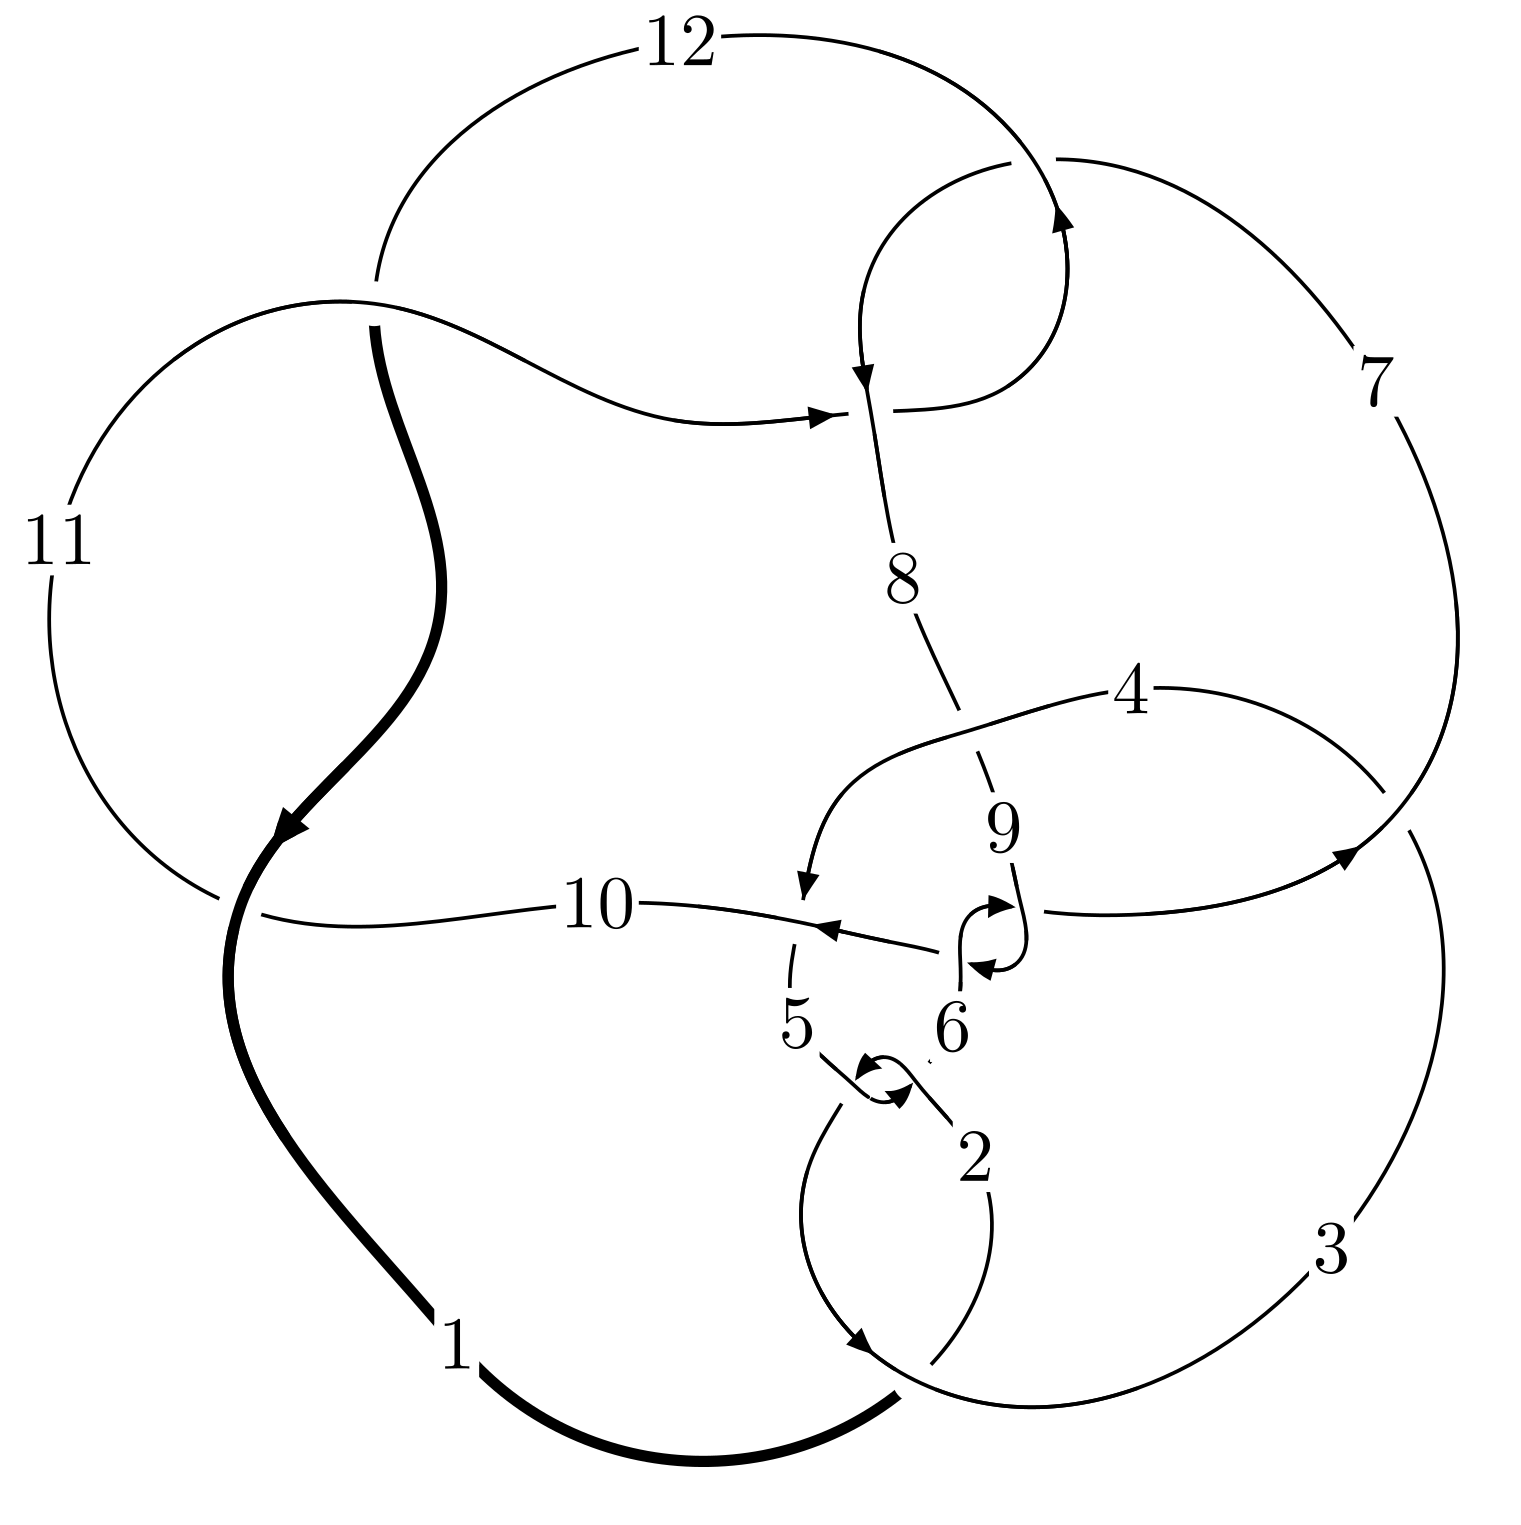
\includegraphics[width=112pt]{../../../GIT/diagram.site/Diagrams/png/874_12a_0073.png}\\
\ \ \ A knot diagram\footnotemark}&
\allowdisplaybreaks
\textbf{Linearized knot diagam} \\
\cline{2-2}
 &
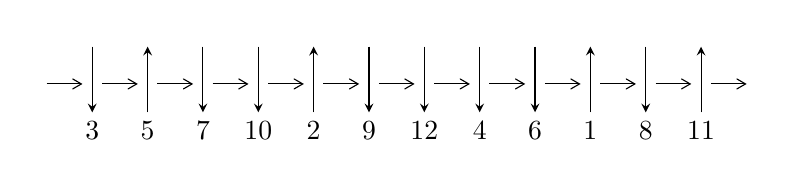
\begin{tikzpicture}[x=20pt, y=17pt]
	% nodes
	\node (C0) at (0, 0) {};
	\node (C1) at (1, 0) {};
	\node (C1U) at (1, +1) {};
	\node (C1D) at (1, -1) {3};

	\node (C2) at (2, 0) {};
	\node (C2U) at (2, +1) {};
	\node (C2D) at (2, -1) {5};

	\node (C3) at (3, 0) {};
	\node (C3U) at (3, +1) {};
	\node (C3D) at (3, -1) {7};

	\node (C4) at (4, 0) {};
	\node (C4U) at (4, +1) {};
	\node (C4D) at (4, -1) {10};

	\node (C5) at (5, 0) {};
	\node (C5U) at (5, +1) {};
	\node (C5D) at (5, -1) {2};

	\node (C6) at (6, 0) {};
	\node (C6U) at (6, +1) {};
	\node (C6D) at (6, -1) {9};

	\node (C7) at (7, 0) {};
	\node (C7U) at (7, +1) {};
	\node (C7D) at (7, -1) {12};

	\node (C8) at (8, 0) {};
	\node (C8U) at (8, +1) {};
	\node (C8D) at (8, -1) {4};

	\node (C9) at (9, 0) {};
	\node (C9U) at (9, +1) {};
	\node (C9D) at (9, -1) {6};

	\node (C10) at (10, 0) {};
	\node (C10U) at (10, +1) {};
	\node (C10D) at (10, -1) {1};

	\node (C11) at (11, 0) {};
	\node (C11U) at (11, +1) {};
	\node (C11D) at (11, -1) {8};

	\node (C12) at (12, 0) {};
	\node (C12U) at (12, +1) {};
	\node (C12D) at (12, -1) {11};
	\node (C13) at (13, 0) {};

	% arrows
	\draw[->,>={angle 60}]
	(C0) edge (C1) (C1) edge (C2) (C2) edge (C3) (C3) edge (C4) (C4) edge (C5) (C5) edge (C6) (C6) edge (C7) (C7) edge (C8) (C8) edge (C9) (C9) edge (C10) (C10) edge (C11) (C11) edge (C12) (C12) edge (C13) ;	\draw[->,>=stealth]
	(C1U) edge (C1D) (C2D) edge (C2U) (C3U) edge (C3D) (C4U) edge (C4D) (C5D) edge (C5U) (C6U) edge (C6D) (C7U) edge (C7D) (C8U) edge (C8D) (C9U) edge (C9D) (C10D) edge (C10U) (C11U) edge (C11D) (C12D) edge (C12U) ;
	\end{tikzpicture} \\
\hhline{~~} \\& 
\textbf{Solving Sequence} \\ \cline{2-2} 
 &
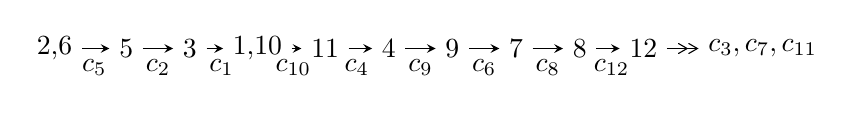
\begin{tikzpicture}[x=23pt, y=7pt]
	% node
	\node (A0) at (-1/8, 0) {2,6};
	\node (A1) at (1, 0) {5};
	\node (A2) at (2, 0) {3};
	\node (A3) at (49/16, 0) {1,10};
	\node (A4) at (33/8, 0) {11};
	\node (A5) at (41/8, 0) {4};
	\node (A6) at (49/8, 0) {9};
	\node (A7) at (57/8, 0) {7};
	\node (A8) at (65/8, 0) {8};
	\node (A9) at (73/8, 0) {12};
	\node (C1) at (1/2, -1) {$c_{5}$};
	\node (C2) at (3/2, -1) {$c_{2}$};
	\node (C3) at (5/2, -1) {$c_{1}$};
	\node (C4) at (29/8, -1) {$c_{10}$};
	\node (C5) at (37/8, -1) {$c_{4}$};
	\node (C6) at (45/8, -1) {$c_{9}$};
	\node (C7) at (53/8, -1) {$c_{6}$};
	\node (C8) at (61/8, -1) {$c_{8}$};
	\node (C9) at (69/8, -1) {$c_{12}$};
	\node (A10) at (11, 0) {$c_{3},c_{7},c_{11}$};

	% edge
	\draw[->,>=stealth]	
	(A0) edge (A1) (A1) edge (A2) (A2) edge (A3) (A3) edge (A4) (A4) edge (A5) (A5) edge (A6) (A6) edge (A7) (A7) edge (A8) (A8) edge (A9) ;
	\draw[->>,>={angle 60}]	
	(A9) edge (A10);
\end{tikzpicture} \\ 

\end{tabular} \\

\footnotetext{
The image of knot diagram is generated by the software ``\textbf{Draw programme}" developed by Andrew Bartholomew(\url{http://www.layer8.co.uk/maths/draw/index.htm\#Running-draw}), where we modified some parts for our purpose(\url{https://github.com/CATsTAILs/LinksPainter}).
}\phantom \\ \newline 
\centering \textbf{Ideals for irreducible components\footnotemark of $X_{\text{par}}$} 
 
\begin{align*}
I^u_{1}&=\langle 
7.66892\times10^{214} u^{104}-5.54270\times10^{214} u^{103}+\cdots+8.78552\times10^{214} b-2.62937\times10^{214},\\
\phantom{I^u_{1}}&\phantom{= \langle  }-7.70789\times10^{214} u^{104}-9.86900\times10^{214} u^{103}+\cdots+8.78552\times10^{214} a-3.93480\times10^{215},\\
\phantom{I^u_{1}}&\phantom{= \langle  }u^{105}+u^{104}+\cdots+3 u+1\rangle \\
\\
\end{align*}
\raggedright * 1 irreducible components of $\dim_{\mathbb{C}}=0$, with total 105 representations.\\
\footnotetext{All coefficients of polynomials are rational numbers. But the coefficients are sometimes approximated in decimal forms when there is not enough margin.}
\newpage
\renewcommand{\arraystretch}{1}
\centering \section*{I. $I^u_{1}= \langle 7.67\times10^{214} u^{104}-5.54\times10^{214} u^{103}+\cdots+8.79\times10^{214} b-2.63\times10^{214},\;-7.71\times10^{214} u^{104}-9.87\times10^{214} u^{103}+\cdots+8.79\times10^{214} a-3.93\times10^{215},\;u^{105}+u^{104}+\cdots+3 u+1 \rangle$}
\flushleft \textbf{(i) Arc colorings}\\
\begin{tabular}{m{7pt} m{180pt} m{7pt} m{180pt} }
\flushright $a_{2}=$&$\begin{pmatrix}0\\u\end{pmatrix}$ \\
\flushright $a_{6}=$&$\begin{pmatrix}1\\0\end{pmatrix}$ \\
\flushright $a_{5}=$&$\begin{pmatrix}1\\u^2\end{pmatrix}$ \\
\flushright $a_{3}=$&$\begin{pmatrix}u\\u^3+u\end{pmatrix}$ \\
\flushright $a_{1}=$&$\begin{pmatrix}u^3\\u^5+u^3+u\end{pmatrix}$ \\
\flushright $a_{10}=$&$\begin{pmatrix}0.877340 u^{104}+1.12333 u^{103}+\cdots-4.89904 u+4.47874\\-0.872905 u^{104}+0.630891 u^{103}+\cdots-2.07805 u+0.299284\end{pmatrix}$ \\
\flushright $a_{11}=$&$\begin{pmatrix}-0.214388 u^{104}+1.49205 u^{103}+\cdots-4.86698 u+4.98395\\-0.608798 u^{104}+0.442648 u^{103}+\cdots-2.47648 u+0.150688\end{pmatrix}$ \\
\flushright $a_{4}=$&$\begin{pmatrix}-2.51175 u^{104}-2.39463 u^{103}+\cdots+10.4331 u+4.89572\\-0.0579607 u^{104}-0.975123 u^{103}+\cdots-3.10564 u-0.356969\end{pmatrix}$ \\
\flushright $a_{9}=$&$\begin{pmatrix}0.00443566 u^{104}+1.75422 u^{103}+\cdots-6.97708 u+4.77802\\-0.872905 u^{104}+0.630891 u^{103}+\cdots-2.07805 u+0.299284\end{pmatrix}$ \\
\flushright $a_{7}=$&$\begin{pmatrix}-2.21119 u^{104}-1.97819 u^{103}+\cdots-8.95378 u-4.10035\\0.647194 u^{104}-1.16684 u^{103}+\cdots-0.177061 u-1.69006\end{pmatrix}$ \\
\flushright $a_{8}=$&$\begin{pmatrix}0.0758079 u^{104}+1.33160 u^{103}+\cdots-5.78845 u+6.83418\\-1.04456 u^{104}+0.913641 u^{103}+\cdots-3.12835 u+0.562654\end{pmatrix}$ \\
\flushright $a_{12}=$&$\begin{pmatrix}-2.58052 u^{104}-1.81430 u^{103}+\cdots-14.5209 u-2.88953\\0.434434 u^{104}-0.542417 u^{103}+\cdots-0.463397 u-1.49524\end{pmatrix}$\\&\end{tabular}
\flushleft \textbf{(ii) Obstruction class $= -1$}\\~\\
\flushleft \textbf{(iii) Cusp Shapes $= 1.26566 u^{104}-6.31791 u^{103}+\cdots+10.2404 u-6.23126$}\\~\\
\newpage\renewcommand{\arraystretch}{1}
\flushleft \textbf{(iv) u-Polynomials at the component}\newline \\
\begin{tabular}{m{50pt}|m{274pt}}
Crossings & \hspace{64pt}u-Polynomials at each crossing \\
\hline $$\begin{aligned}c_{1}\end{aligned}$$&$\begin{aligned}
&u^{105}+43 u^{104}+\cdots-7 u-1
\end{aligned}$\\
\hline $$\begin{aligned}c_{2},c_{5}\end{aligned}$$&$\begin{aligned}
&u^{105}+u^{104}+\cdots+3 u+1
\end{aligned}$\\
\hline $$\begin{aligned}c_{3}\end{aligned}$$&$\begin{aligned}
&u^{105}-27 u^{104}+\cdots-9 u+1
\end{aligned}$\\
\hline $$\begin{aligned}c_{4}\end{aligned}$$&$\begin{aligned}
&u^{105}-15 u^{104}+\cdots+15789 u+52699
\end{aligned}$\\
\hline $$\begin{aligned}c_{6},c_{9}\end{aligned}$$&$\begin{aligned}
&u^{105}-5 u^{104}+\cdots-3 u+1
\end{aligned}$\\
\hline $$\begin{aligned}c_{7},c_{11}\end{aligned}$$&$\begin{aligned}
&u^{105}+5 u^{104}+\cdots- u+1
\end{aligned}$\\
\hline $$\begin{aligned}c_{8}\end{aligned}$$&$\begin{aligned}
&u^{105}- u^{104}+\cdots-11 u+1
\end{aligned}$\\
\hline $$\begin{aligned}c_{10},c_{12}\end{aligned}$$&$\begin{aligned}
&u^{105}-31 u^{104}+\cdots+5 u+1
\end{aligned}$\\
\hline
\end{tabular}\\~\\
\newpage\renewcommand{\arraystretch}{1}
\flushleft \textbf{(v) Riley Polynomials at the component}\newline \\
\begin{tabular}{m{50pt}|m{274pt}}
Crossings & \hspace{64pt}Riley Polynomials at each crossing \\
\hline $$\begin{aligned}c_{1}\end{aligned}$$&$\begin{aligned}
&y^{105}+39 y^{104}+\cdots-579 y-1
\end{aligned}$\\
\hline $$\begin{aligned}c_{2},c_{5}\end{aligned}$$&$\begin{aligned}
&y^{105}+43 y^{104}+\cdots-7 y-1
\end{aligned}$\\
\hline $$\begin{aligned}c_{3}\end{aligned}$$&$\begin{aligned}
&y^{105}+95 y^{104}+\cdots-295 y-1
\end{aligned}$\\
\hline $$\begin{aligned}c_{4}\end{aligned}$$&$\begin{aligned}
&y^{105}-17 y^{104}+\cdots+26937541693 y-2777184601
\end{aligned}$\\
\hline $$\begin{aligned}c_{6},c_{9}\end{aligned}$$&$\begin{aligned}
&y^{105}+75 y^{104}+\cdots+5 y-1
\end{aligned}$\\
\hline $$\begin{aligned}c_{7},c_{11}\end{aligned}$$&$\begin{aligned}
&y^{105}+31 y^{104}+\cdots+5 y-1
\end{aligned}$\\
\hline $$\begin{aligned}c_{8}\end{aligned}$$&$\begin{aligned}
&y^{105}-5 y^{104}+\cdots+33 y-1
\end{aligned}$\\
\hline $$\begin{aligned}c_{10},c_{12}\end{aligned}$$&$\begin{aligned}
&y^{105}+87 y^{104}+\cdots-251 y-1
\end{aligned}$\\
\hline
\end{tabular}\\~\\
\newpage\flushleft \textbf{(vi) Complex Volumes and Cusp Shapes}
$$\begin{array}{c|c|c}  
\text{Solutions to }I^u_{1}& \I (\text{vol} + \sqrt{-1}CS) & \text{Cusp shape}\\
 \hline 
\begin{aligned}
u &= \phantom{-}0.508255 + 0.862936 I \\
a &= \phantom{-}7.42480 + 9.85920 I \\
b &= -0.027672 - 0.963307 I\end{aligned}
 & -1.35091 + 4.86008 I & \phantom{-0.000000 } 0 \\ \hline\begin{aligned}
u &= \phantom{-}0.508255 - 0.862936 I \\
a &= \phantom{-}7.42480 - 9.85920 I \\
b &= -0.027672 + 0.963307 I\end{aligned}
 & -1.35091 - 4.86008 I & \phantom{-0.000000 } 0 \\ \hline\begin{aligned}
u &= -0.726437 + 0.681228 I \\
a &= \phantom{-}0.302847 - 0.123414 I \\
b &= \phantom{-}0.41559 - 1.45271 I\end{aligned}
 & \phantom{-}7.14004 - 0.17018 I & \phantom{-0.000000 } 0 \\ \hline\begin{aligned}
u &= -0.726437 - 0.681228 I \\
a &= \phantom{-}0.302847 + 0.123414 I \\
b &= \phantom{-}0.41559 + 1.45271 I\end{aligned}
 & \phantom{-}7.14004 + 0.17018 I & \phantom{-0.000000 } 0 \\ \hline\begin{aligned}
u &= \phantom{-}0.670011 + 0.735882 I \\
a &= -0.398917 + 1.060470 I \\
b &= \phantom{-}0.218711 - 0.343183 I\end{aligned}
 & -1.53322 + 5.27277 I & \phantom{-0.000000 } 0 \\ \hline\begin{aligned}
u &= \phantom{-}0.670011 - 0.735882 I \\
a &= -0.398917 - 1.060470 I \\
b &= \phantom{-}0.218711 + 0.343183 I\end{aligned}
 & -1.53322 - 5.27277 I & \phantom{-0.000000 } 0 \\ \hline\begin{aligned}
u &= \phantom{-}0.498514 + 0.873517 I \\
a &= -13.15460 + 0.69616 I \\
b &= \phantom{-}0.039933 + 1.006260 I\end{aligned}
 & -1.39472 - 0.77663 I & \phantom{-0.000000 } 0 \\ \hline\begin{aligned}
u &= \phantom{-}0.498514 - 0.873517 I \\
a &= -13.15460 - 0.69616 I \\
b &= \phantom{-}0.039933 - 1.006260 I\end{aligned}
 & -1.39472 + 0.77663 I & \phantom{-0.000000 } 0 \\ \hline\begin{aligned}
u &= \phantom{-}0.416633 + 0.881483 I \\
a &= -0.697391 - 0.189517 I \\
b &= \phantom{-}0.218983 + 0.169046 I\end{aligned}
 & -0.33676 + 1.74914 I & \phantom{-0.000000 } 0 \\ \hline\begin{aligned}
u &= \phantom{-}0.416633 - 0.881483 I \\
a &= -0.697391 + 0.189517 I \\
b &= \phantom{-}0.218983 - 0.169046 I\end{aligned}
 & -0.33676 - 1.74914 I & \phantom{-0.000000 } 0\\
 \hline 
 \end{array}$$\newpage$$\begin{array}{c|c|c}  
\text{Solutions to }I^u_{1}& \I (\text{vol} + \sqrt{-1}CS) & \text{Cusp shape}\\
 \hline 
\begin{aligned}
u &= -0.421508 + 0.941394 I \\
a &= \phantom{-}0.113393 - 1.188910 I \\
b &= -0.88553 + 1.17946 I\end{aligned}
 & -2.90888 - 0.14378 I & \phantom{-0.000000 } 0 \\ \hline\begin{aligned}
u &= -0.421508 - 0.941394 I \\
a &= \phantom{-}0.113393 + 1.188910 I \\
b &= -0.88553 - 1.17946 I\end{aligned}
 & -2.90888 + 0.14378 I & \phantom{-0.000000 } 0 \\ \hline\begin{aligned}
u &= -0.000183 + 1.041080 I \\
a &= \phantom{-}0.655071 - 1.227110 I \\
b &= -0.461490 + 0.982731 I\end{aligned}
 & -1.37985 + 2.60061 I & \phantom{-0.000000 } 0 \\ \hline\begin{aligned}
u &= -0.000183 - 1.041080 I \\
a &= \phantom{-}0.655071 + 1.227110 I \\
b &= -0.461490 - 0.982731 I\end{aligned}
 & -1.37985 - 2.60061 I & \phantom{-0.000000 } 0 \\ \hline\begin{aligned}
u &= -0.462542 + 0.937742 I \\
a &= \phantom{-}2.01181 - 0.08750 I \\
b &= -0.38997 - 1.69307 I\end{aligned}
 & -2.72043 - 5.15393 I & \phantom{-0.000000 } 0 \\ \hline\begin{aligned}
u &= -0.462542 - 0.937742 I \\
a &= \phantom{-}2.01181 + 0.08750 I \\
b &= -0.38997 + 1.69307 I\end{aligned}
 & -2.72043 + 5.15393 I & \phantom{-0.000000 } 0 \\ \hline\begin{aligned}
u &= -0.944508 + 0.449202 I \\
a &= \phantom{-}0.227674 + 0.414665 I \\
b &= -0.43011 + 1.35679 I\end{aligned}
 & \phantom{-}0.58537 + 6.60149 I & \phantom{-0.000000 } 0 \\ \hline\begin{aligned}
u &= -0.944508 - 0.449202 I \\
a &= \phantom{-}0.227674 - 0.414665 I \\
b &= -0.43011 - 1.35679 I\end{aligned}
 & \phantom{-}0.58537 - 6.60149 I & \phantom{-0.000000 } 0 \\ \hline\begin{aligned}
u &= \phantom{-}0.673932 + 0.800679 I \\
a &= \phantom{-}0.449328 - 0.906610 I \\
b &= -0.236551 + 0.292446 I\end{aligned}
 & -1.68329 - 0.14385 I & \phantom{-0.000000 } 0 \\ \hline\begin{aligned}
u &= \phantom{-}0.673932 - 0.800679 I \\
a &= \phantom{-}0.449328 + 0.906610 I \\
b &= -0.236551 - 0.292446 I\end{aligned}
 & -1.68329 + 0.14385 I & \phantom{-0.000000 } 0\\
 \hline 
 \end{array}$$\newpage$$\begin{array}{c|c|c}  
\text{Solutions to }I^u_{1}& \I (\text{vol} + \sqrt{-1}CS) & \text{Cusp shape}\\
 \hline 
\begin{aligned}
u &= -0.420652 + 0.958376 I \\
a &= \phantom{-}1.60412 - 0.80365 I \\
b &= -1.169270 - 0.420460 I\end{aligned}
 & -2.94183 - 2.82687 I & \phantom{-0.000000 } 0 \\ \hline\begin{aligned}
u &= -0.420652 - 0.958376 I \\
a &= \phantom{-}1.60412 + 0.80365 I \\
b &= -1.169270 + 0.420460 I\end{aligned}
 & -2.94183 + 2.82687 I & \phantom{-0.000000 } 0 \\ \hline\begin{aligned}
u &= -0.406993 + 0.861247 I \\
a &= -1.79250 + 0.05635 I \\
b &= \phantom{-}0.11232 + 1.69617 I\end{aligned}
 & -2.32293 + 1.64088 I & \phantom{-0.000000 } 0 \\ \hline\begin{aligned}
u &= -0.406993 - 0.861247 I \\
a &= -1.79250 - 0.05635 I \\
b &= \phantom{-}0.11232 - 1.69617 I\end{aligned}
 & -2.32293 - 1.64088 I & \phantom{-0.000000 } 0 \\ \hline\begin{aligned}
u &= -0.883123 + 0.572875 I \\
a &= -0.048849 - 0.279960 I \\
b &= \phantom{-}0.42862 - 1.38709 I\end{aligned}
 & \phantom{-}7.89421 + 6.86350 I & \phantom{-0.000000 } 0 \\ \hline\begin{aligned}
u &= -0.883123 - 0.572875 I \\
a &= -0.048849 + 0.279960 I \\
b &= \phantom{-}0.42862 + 1.38709 I\end{aligned}
 & \phantom{-}7.89421 - 6.86350 I & \phantom{-0.000000 } 0 \\ \hline\begin{aligned}
u &= \phantom{-}0.604807 + 0.709411 I \\
a &= -0.06549 + 1.57847 I \\
b &= -0.034649 + 1.142580 I\end{aligned}
 & \phantom{-}3.17185 + 1.49000 I & \phantom{-0.000000 } 0 \\ \hline\begin{aligned}
u &= \phantom{-}0.604807 - 0.709411 I \\
a &= -0.06549 - 1.57847 I \\
b &= -0.034649 - 1.142580 I\end{aligned}
 & \phantom{-}3.17185 - 1.49000 I & \phantom{-0.000000 } 0 \\ \hline\begin{aligned}
u &= -0.758524 + 0.535990 I \\
a &= -0.154021 + 0.433594 I \\
b &= -0.39001 + 1.39514 I\end{aligned}
 & \phantom{-}3.99639 + 3.72302 I & \phantom{-0.000000 } 0 \\ \hline\begin{aligned}
u &= -0.758524 - 0.535990 I \\
a &= -0.154021 - 0.433594 I \\
b &= -0.39001 - 1.39514 I\end{aligned}
 & \phantom{-}3.99639 - 3.72302 I & \phantom{-0.000000 } 0\\
 \hline 
 \end{array}$$\newpage$$\begin{array}{c|c|c}  
\text{Solutions to }I^u_{1}& \I (\text{vol} + \sqrt{-1}CS) & \text{Cusp shape}\\
 \hline 
\begin{aligned}
u &= -0.524210 + 0.945636 I \\
a &= \phantom{-}0.190673 + 0.999026 I \\
b &= \phantom{-}0.80345 - 1.44636 I\end{aligned}
 & -1.36172 - 6.40994 I & \phantom{-0.000000 } 0 \\ \hline\begin{aligned}
u &= -0.524210 - 0.945636 I \\
a &= \phantom{-}0.190673 - 0.999026 I \\
b &= \phantom{-}0.80345 + 1.44636 I\end{aligned}
 & -1.36172 + 6.40994 I & \phantom{-0.000000 } 0 \\ \hline\begin{aligned}
u &= -0.978052 + 0.472820 I \\
a &= -0.250397 - 0.357539 I \\
b &= \phantom{-}0.43741 - 1.35953 I\end{aligned}
 & \phantom{-}1.51311 + 12.62850 I & \phantom{-0.000000 } 0 \\ \hline\begin{aligned}
u &= -0.978052 - 0.472820 I \\
a &= -0.250397 + 0.357539 I \\
b &= \phantom{-}0.43741 + 1.35953 I\end{aligned}
 & \phantom{-}1.51311 - 12.62850 I & \phantom{-0.000000 } 0 \\ \hline\begin{aligned}
u &= -0.786078 + 0.399159 I \\
a &= -0.422992 + 0.480443 I \\
b &= \phantom{-}0.929515 - 0.138087 I\end{aligned}
 & -3.14157 + 7.73150 I & \phantom{-0.000000 } 0 \\ \hline\begin{aligned}
u &= -0.786078 - 0.399159 I \\
a &= -0.422992 - 0.480443 I \\
b &= \phantom{-}0.929515 + 0.138087 I\end{aligned}
 & -3.14157 - 7.73150 I & \phantom{-0.000000 } 0 \\ \hline\begin{aligned}
u &= \phantom{-}0.101092 + 0.874217 I \\
a &= -1.52874 - 0.02687 I \\
b &= \phantom{-}0.509118 + 0.386326 I\end{aligned}
 & -1.22927 + 1.94221 I & \phantom{-0.000000 } 0 \\ \hline\begin{aligned}
u &= \phantom{-}0.101092 - 0.874217 I \\
a &= -1.52874 + 0.02687 I \\
b &= \phantom{-}0.509118 - 0.386326 I\end{aligned}
 & -1.22927 - 1.94221 I & \phantom{-0.000000 } 0 \\ \hline\begin{aligned}
u &= \phantom{-}0.572492 + 0.963051 I \\
a &= \phantom{-}0.618677 - 0.447757 I \\
b &= -0.289709 + 0.100685 I\end{aligned}
 & \phantom{-}1.38092 + 3.06411 I & \phantom{-0.000000 } 0 \\ \hline\begin{aligned}
u &= \phantom{-}0.572492 - 0.963051 I \\
a &= \phantom{-}0.618677 + 0.447757 I \\
b &= -0.289709 - 0.100685 I\end{aligned}
 & \phantom{-}1.38092 - 3.06411 I & \phantom{-0.000000 } 0\\
 \hline 
 \end{array}$$\newpage$$\begin{array}{c|c|c}  
\text{Solutions to }I^u_{1}& \I (\text{vol} + \sqrt{-1}CS) & \text{Cusp shape}\\
 \hline 
\begin{aligned}
u &= -0.577256 + 0.970351 I \\
a &= -1.24254 + 0.92560 I \\
b &= \phantom{-}1.265650 + 0.082613 I\end{aligned}
 & \phantom{-}1.68086 - 6.53955 I & \phantom{-0.000000 } 0 \\ \hline\begin{aligned}
u &= -0.577256 - 0.970351 I \\
a &= -1.24254 - 0.92560 I \\
b &= \phantom{-}1.265650 - 0.082613 I\end{aligned}
 & \phantom{-}1.68086 + 6.53955 I & \phantom{-0.000000 } 0 \\ \hline\begin{aligned}
u &= \phantom{-}1.133270 + 0.094508 I \\
a &= -0.0108772 - 0.1312870 I \\
b &= \phantom{-}0.008558 - 1.226130 I\end{aligned}
 & \phantom{-}3.44061 - 2.55226 I & \phantom{-0.000000 } 0 \\ \hline\begin{aligned}
u &= \phantom{-}1.133270 - 0.094508 I \\
a &= -0.0108772 + 0.1312870 I \\
b &= \phantom{-}0.008558 + 1.226130 I\end{aligned}
 & \phantom{-}3.44061 + 2.55226 I & \phantom{-0.000000 } 0 \\ \hline\begin{aligned}
u &= -0.443283 + 0.714059 I \\
a &= -2.00536 + 0.69393 I \\
b &= \phantom{-}0.845499 + 0.998451 I\end{aligned}
 & -0.58409 + 2.30355 I & \phantom{-0.000000 } 0 \\ \hline\begin{aligned}
u &= -0.443283 - 0.714059 I \\
a &= -2.00536 - 0.69393 I \\
b &= \phantom{-}0.845499 - 0.998451 I\end{aligned}
 & -0.58409 - 2.30355 I & \phantom{-0.000000 } 0 \\ \hline\begin{aligned}
u &= \phantom{-}1.062760 + 0.471860 I \\
a &= -0.118414 - 0.270868 I \\
b &= \phantom{-}0.044239 - 1.215040 I\end{aligned}
 & \phantom{-}6.76585 + 1.83284 I & \phantom{-0.000000 } 0 \\ \hline\begin{aligned}
u &= \phantom{-}1.062760 - 0.471860 I \\
a &= -0.118414 + 0.270868 I \\
b &= \phantom{-}0.044239 + 1.215040 I\end{aligned}
 & \phantom{-}6.76585 - 1.83284 I & \phantom{-0.000000 } 0 \\ \hline\begin{aligned}
u &= -0.651366 + 0.971836 I \\
a &= -1.92468 + 0.26060 I \\
b &= \phantom{-}0.59797 + 1.44518 I\end{aligned}
 & \phantom{-}6.25598 - 5.09845 I & \phantom{-0.000000 } 0 \\ \hline\begin{aligned}
u &= -0.651366 - 0.971836 I \\
a &= -1.92468 - 0.26060 I \\
b &= \phantom{-}0.59797 - 1.44518 I\end{aligned}
 & \phantom{-}6.25598 + 5.09845 I & \phantom{-0.000000 } 0\\
 \hline 
 \end{array}$$\newpage$$\begin{array}{c|c|c}  
\text{Solutions to }I^u_{1}& \I (\text{vol} + \sqrt{-1}CS) & \text{Cusp shape}\\
 \hline 
\begin{aligned}
u &= -0.557017 + 0.613871 I \\
a &= -0.409467 + 0.939341 I \\
b &= \phantom{-}0.987950 - 0.342672 I\end{aligned}
 & \phantom{-}2.71513 + 1.93385 I & \phantom{-0.000000 } 0 \\ \hline\begin{aligned}
u &= -0.557017 - 0.613871 I \\
a &= -0.409467 - 0.939341 I \\
b &= \phantom{-}0.987950 + 0.342672 I\end{aligned}
 & \phantom{-}2.71513 - 1.93385 I & \phantom{-0.000000 } 0 \\ \hline\begin{aligned}
u &= -0.747186 + 0.332399 I \\
a &= \phantom{-}0.332745 - 0.437546 I \\
b &= -0.896635 + 0.130466 I\end{aligned}
 & -4.04595 + 1.81268 I & \phantom{-0.000000 } 0 \\ \hline\begin{aligned}
u &= -0.747186 - 0.332399 I \\
a &= \phantom{-}0.332745 + 0.437546 I \\
b &= -0.896635 - 0.130466 I\end{aligned}
 & -4.04595 - 1.81268 I & \phantom{-0.000000 } 0 \\ \hline\begin{aligned}
u &= \phantom{-}0.622436 + 1.009490 I \\
a &= -1.69807 - 0.26278 I \\
b &= \phantom{-}0.139745 - 1.105790 I\end{aligned}
 & \phantom{-}2.09705 + 3.42836 I & \phantom{-0.000000 } 0 \\ \hline\begin{aligned}
u &= \phantom{-}0.622436 - 1.009490 I \\
a &= -1.69807 + 0.26278 I \\
b &= \phantom{-}0.139745 + 1.105790 I\end{aligned}
 & \phantom{-}2.09705 - 3.42836 I & \phantom{-0.000000 } 0 \\ \hline\begin{aligned}
u &= -0.181525 + 1.172900 I \\
a &= \phantom{-}1.42896 - 0.46621 I \\
b &= -0.829191 - 0.232875 I\end{aligned}
 & -8.82234 - 0.91544 I & \phantom{-0.000000 } 0 \\ \hline\begin{aligned}
u &= -0.181525 - 1.172900 I \\
a &= \phantom{-}1.42896 + 0.46621 I \\
b &= -0.829191 + 0.232875 I\end{aligned}
 & -8.82234 + 0.91544 I & \phantom{-0.000000 } 0 \\ \hline\begin{aligned}
u &= \phantom{-}0.456154 + 0.664711 I \\
a &= \phantom{-}0.61525 + 1.56775 I \\
b &= -0.020906 - 0.518366 I\end{aligned}
 & \phantom{-}2.33820 + 1.37333 I & \phantom{-0.000000 } 0 \\ \hline\begin{aligned}
u &= \phantom{-}0.456154 - 0.664711 I \\
a &= \phantom{-}0.61525 - 1.56775 I \\
b &= -0.020906 + 0.518366 I\end{aligned}
 & \phantom{-}2.33820 - 1.37333 I & \phantom{-0.000000 } 0\\
 \hline 
 \end{array}$$\newpage$$\begin{array}{c|c|c}  
\text{Solutions to }I^u_{1}& \I (\text{vol} + \sqrt{-1}CS) & \text{Cusp shape}\\
 \hline 
\begin{aligned}
u &= -0.133227 + 1.187360 I \\
a &= -1.41101 + 0.43669 I \\
b &= \phantom{-}0.795493 + 0.218832 I\end{aligned}
 & -8.34685 + 5.22128 I & \phantom{-0.000000 } 0 \\ \hline\begin{aligned}
u &= -0.133227 - 1.187360 I \\
a &= -1.41101 - 0.43669 I \\
b &= \phantom{-}0.795493 - 0.218832 I\end{aligned}
 & -8.34685 - 5.22128 I & \phantom{-0.000000 } 0 \\ \hline\begin{aligned}
u &= \phantom{-}0.477886 + 1.111110 I \\
a &= -0.927862 + 0.357458 I \\
b &= \phantom{-}0.433014 - 0.015021 I\end{aligned}
 & -3.85790 + 1.05487 I & \phantom{-0.000000 } 0 \\ \hline\begin{aligned}
u &= \phantom{-}0.477886 - 1.111110 I \\
a &= -0.927862 - 0.357458 I \\
b &= \phantom{-}0.433014 + 0.015021 I\end{aligned}
 & -3.85790 - 1.05487 I & \phantom{-0.000000 } 0 \\ \hline\begin{aligned}
u &= \phantom{-}0.522546 + 1.107910 I \\
a &= \phantom{-}0.895110 - 0.406895 I \\
b &= -0.423129 + 0.048731 I\end{aligned}
 & -3.53406 + 6.74367 I & \phantom{-0.000000 } 0 \\ \hline\begin{aligned}
u &= \phantom{-}0.522546 - 1.107910 I \\
a &= \phantom{-}0.895110 + 0.406895 I \\
b &= -0.423129 - 0.048731 I\end{aligned}
 & -3.53406 - 6.74367 I & \phantom{-0.000000 } 0 \\ \hline\begin{aligned}
u &= \phantom{-}0.195343 + 1.213140 I \\
a &= -0.955707 + 0.975328 I \\
b &= \phantom{-}0.347571 - 1.069600 I\end{aligned}
 & \phantom{-}0.76843 + 5.57184 I & \phantom{-0.000000 } 0 \\ \hline\begin{aligned}
u &= \phantom{-}0.195343 - 1.213140 I \\
a &= -0.955707 - 0.975328 I \\
b &= \phantom{-}0.347571 + 1.069600 I\end{aligned}
 & \phantom{-}0.76843 - 5.57184 I & \phantom{-0.000000 } 0 \\ \hline\begin{aligned}
u &= -0.635360 + 1.051860 I \\
a &= \phantom{-}1.91539 - 0.19142 I \\
b &= -0.53909 - 1.43926 I\end{aligned}
 & \phantom{-}2.46261 - 9.01692 I & \phantom{-0.000000 } 0 \\ \hline\begin{aligned}
u &= -0.635360 - 1.051860 I \\
a &= \phantom{-}1.91539 + 0.19142 I \\
b &= -0.53909 + 1.43926 I\end{aligned}
 & \phantom{-}2.46261 + 9.01692 I & \phantom{-0.000000 } 0\\
 \hline 
 \end{array}$$\newpage$$\begin{array}{c|c|c}  
\text{Solutions to }I^u_{1}& \I (\text{vol} + \sqrt{-1}CS) & \text{Cusp shape}\\
 \hline 
\begin{aligned}
u &= -0.573696 + 1.101490 I \\
a &= \phantom{-}1.27872 - 0.73078 I \\
b &= -1.113830 - 0.111897 I\end{aligned}
 & -6.25145 - 6.77312 I & \phantom{-0.000000 } 0 \\ \hline\begin{aligned}
u &= -0.573696 - 1.101490 I \\
a &= \phantom{-}1.27872 + 0.73078 I \\
b &= -1.113830 + 0.111897 I\end{aligned}
 & -6.25145 + 6.77312 I & \phantom{-0.000000 } 0 \\ \hline\begin{aligned}
u &= -0.607709 + 1.103640 I \\
a &= -1.24531 + 0.72570 I \\
b &= \phantom{-}1.113740 + 0.085690 I\end{aligned}
 & -5.20237 - 12.95960 I & \phantom{-0.000000 } 0 \\ \hline\begin{aligned}
u &= -0.607709 - 1.103640 I \\
a &= -1.24531 - 0.72570 I \\
b &= \phantom{-}1.113740 - 0.085690 I\end{aligned}
 & -5.20237 + 12.95960 I & \phantom{-0.000000 } 0 \\ \hline\begin{aligned}
u &= -0.695529 + 1.076720 I \\
a &= -1.86993 + 0.18482 I \\
b &= \phantom{-}0.54253 + 1.40519 I\end{aligned}
 & \phantom{-}6.3495 - 12.6969 I & \phantom{-0.000000 } 0 \\ \hline\begin{aligned}
u &= -0.695529 - 1.076720 I \\
a &= -1.86993 - 0.18482 I \\
b &= \phantom{-}0.54253 - 1.40519 I\end{aligned}
 & \phantom{-}6.3495 + 12.6969 I & \phantom{-0.000000 } 0 \\ \hline\begin{aligned}
u &= \phantom{-}0.604480 + 0.379071 I \\
a &= -0.551150 + 0.357450 I \\
b &= -0.018965 + 1.181400 I\end{aligned}
 & \phantom{-}3.35286 + 1.30846 I & -2.29563 - 4.32140 I \\ \hline\begin{aligned}
u &= \phantom{-}0.604480 - 0.379071 I \\
a &= -0.551150 - 0.357450 I \\
b &= -0.018965 - 1.181400 I\end{aligned}
 & \phantom{-}3.35286 - 1.30846 I & -2.29563 + 4.32140 I \\ \hline\begin{aligned}
u &= \phantom{-}1.016120 + 0.853696 I \\
a &= \phantom{-}0.519396 + 0.310803 I \\
b &= -0.094416 + 1.202750 I\end{aligned}
 & \phantom{-}2.39877 + 1.01374 I & \phantom{-0.000000 } 0 \\ \hline\begin{aligned}
u &= \phantom{-}1.016120 - 0.853696 I \\
a &= \phantom{-}0.519396 - 0.310803 I \\
b &= -0.094416 - 1.202750 I\end{aligned}
 & \phantom{-}2.39877 - 1.01374 I & \phantom{-0.000000 } 0\\
 \hline 
 \end{array}$$\newpage$$\begin{array}{c|c|c}  
\text{Solutions to }I^u_{1}& \I (\text{vol} + \sqrt{-1}CS) & \text{Cusp shape}\\
 \hline 
\begin{aligned}
u &= -0.672944 + 1.147260 I \\
a &= \phantom{-}1.87685 - 0.13801 I \\
b &= -0.51403 - 1.39635 I\end{aligned}
 & -1.55003 - 12.50060 I & \phantom{-0.000000 } 0 \\ \hline\begin{aligned}
u &= -0.672944 - 1.147260 I \\
a &= \phantom{-}1.87685 + 0.13801 I \\
b &= -0.51403 + 1.39635 I\end{aligned}
 & -1.55003 + 12.50060 I & \phantom{-0.000000 } 0 \\ \hline\begin{aligned}
u &= \phantom{-}1.094560 + 0.763773 I \\
a &= -0.387061 - 0.268070 I \\
b &= \phantom{-}0.080994 - 1.214740 I\end{aligned}
 & \phantom{-}2.71739 + 6.28347 I & \phantom{-0.000000 } 0 \\ \hline\begin{aligned}
u &= \phantom{-}1.094560 - 0.763773 I \\
a &= -0.387061 + 0.268070 I \\
b &= \phantom{-}0.080994 + 1.214740 I\end{aligned}
 & \phantom{-}2.71739 - 6.28347 I & \phantom{-0.000000 } 0 \\ \hline\begin{aligned}
u &= -0.016022 + 1.345400 I \\
a &= \phantom{-}0.689201 - 0.878906 I \\
b &= -0.426397 + 1.135310 I\end{aligned}
 & -6.05046 + 3.63906 I & \phantom{-0.000000 } 0 \\ \hline\begin{aligned}
u &= -0.016022 - 1.345400 I \\
a &= \phantom{-}0.689201 + 0.878906 I \\
b &= -0.426397 - 1.135310 I\end{aligned}
 & -6.05046 - 3.63906 I & \phantom{-0.000000 } 0 \\ \hline\begin{aligned}
u &= -0.692371 + 1.153980 I \\
a &= -1.86487 + 0.13570 I \\
b &= \phantom{-}0.51713 + 1.38967 I\end{aligned}
 & -0.5913 - 18.6960 I & \phantom{-0.000000 } 0 \\ \hline\begin{aligned}
u &= -0.692371 - 1.153980 I \\
a &= -1.86487 - 0.13570 I \\
b &= \phantom{-}0.51713 - 1.38967 I\end{aligned}
 & -0.5913 + 18.6960 I & \phantom{-0.000000 } 0 \\ \hline\begin{aligned}
u &= \phantom{-}0.023126 + 1.377250 I \\
a &= -0.719581 + 0.849284 I \\
b &= \phantom{-}0.409086 - 1.141730 I\end{aligned}
 & -5.52098 + 9.62166 I & \phantom{-0.000000 } 0 \\ \hline\begin{aligned}
u &= \phantom{-}0.023126 - 1.377250 I \\
a &= -0.719581 - 0.849284 I \\
b &= \phantom{-}0.409086 + 1.141730 I\end{aligned}
 & -5.52098 - 9.62166 I & \phantom{-0.000000 } 0\\
 \hline 
 \end{array}$$\newpage$$\begin{array}{c|c|c}  
\text{Solutions to }I^u_{1}& \I (\text{vol} + \sqrt{-1}CS) & \text{Cusp shape}\\
 \hline 
\begin{aligned}
u &= \phantom{-}0.805185 + 1.119210 I \\
a &= \phantom{-}1.009610 + 0.085722 I \\
b &= -0.154249 + 1.170110 I\end{aligned}
 & \phantom{-}4.84892 + 4.84004 I & \phantom{-0.000000 } 0 \\ \hline\begin{aligned}
u &= \phantom{-}0.805185 - 1.119210 I \\
a &= \phantom{-}1.009610 - 0.085722 I \\
b &= -0.154249 - 1.170110 I\end{aligned}
 & \phantom{-}4.84892 - 4.84004 I & \phantom{-0.000000 } 0 \\ \hline\begin{aligned}
u &= \phantom{-}0.272901 + 0.554183 I \\
a &= -0.19275 + 2.00690 I \\
b &= \phantom{-}0.257419 - 0.608789 I\end{aligned}
 & \phantom{-}2.30617 + 1.35689 I & \phantom{-}0.69154 - 4.56259 I \\ \hline\begin{aligned}
u &= \phantom{-}0.272901 - 0.554183 I \\
a &= -0.19275 - 2.00690 I \\
b &= \phantom{-}0.257419 + 0.608789 I\end{aligned}
 & \phantom{-}2.30617 - 1.35689 I & \phantom{-}0.69154 + 4.56259 I \\ \hline\begin{aligned}
u &= \phantom{-}0.65848 + 1.29036 I \\
a &= -1.068220 + 0.283751 I \\
b &= \phantom{-}0.211206 - 1.163030 I\end{aligned}
 & -0.52858 + 3.53870 I & \phantom{-0.000000 } 0 \\ \hline\begin{aligned}
u &= \phantom{-}0.65848 - 1.29036 I \\
a &= -1.068220 - 0.283751 I \\
b &= \phantom{-}0.211206 + 1.163030 I\end{aligned}
 & -0.52858 - 3.53870 I & \phantom{-0.000000 } 0 \\ \hline\begin{aligned}
u &= \phantom{-}0.72220 + 1.29833 I \\
a &= \phantom{-}1.003820 - 0.223822 I \\
b &= -0.201729 + 1.176080 I\end{aligned}
 & -0.06083 + 9.13213 I & \phantom{-0.000000 } 0 \\ \hline\begin{aligned}
u &= \phantom{-}0.72220 - 1.29833 I \\
a &= \phantom{-}1.003820 + 0.223822 I \\
b &= -0.201729 - 1.176080 I\end{aligned}
 & -0.06083 - 9.13213 I & \phantom{-0.000000 } 0 \\ \hline\begin{aligned}
u &= \phantom{-}0.270706 + 0.375679 I \\
a &= \phantom{-}2.42139 + 1.77339 I \\
b &= -0.236524 - 0.659638 I\end{aligned}
 & -1.27823 - 2.63513 I & -5.66825 + 3.44323 I \\ \hline\begin{aligned}
u &= \phantom{-}0.270706 - 0.375679 I \\
a &= \phantom{-}2.42139 - 1.77339 I \\
b &= -0.236524 + 0.659638 I\end{aligned}
 & -1.27823 + 2.63513 I & -5.66825 - 3.44323 I\\
 \hline 
 \end{array}$$\newpage$$\begin{array}{c|c|c}  
\text{Solutions to }I^u_{1}& \I (\text{vol} + \sqrt{-1}CS) & \text{Cusp shape}\\
 \hline 
\begin{aligned}
u &= -0.336905\phantom{ +0.000000I} \\
a &= -0.721891\phantom{ +0.000000I} \\
b &= -0.588949\phantom{ +0.000000I}\end{aligned}
 & -0.940602\phantom{ +0.000000I} & -10.3260\phantom{ +0.000000I} \\ \hline\begin{aligned}
u &= \phantom{-}0.322904 + 0.028835 I \\
a &= -1.17535 - 3.20754 I \\
b &= \phantom{-}0.143408 + 0.600910 I\end{aligned}
 & -1.22625 + 2.67668 I & -4.97081 - 2.18693 I \\ \hline\begin{aligned}
u &= \phantom{-}0.322904 - 0.028835 I \\
a &= -1.17535 + 3.20754 I \\
b &= \phantom{-}0.143408 - 0.600910 I\end{aligned}
 & -1.22625 - 2.67668 I & -4.97081 + 2.18693 I \\ \hline\begin{aligned}
u &= -0.141033 + 0.171770 I \\
a &= \phantom{-}4.56827 - 2.64364 I \\
b &= -0.276321 - 0.948170 I\end{aligned}
 & -1.35507 - 2.65461 I & -5.59031 + 3.22885 I \\ \hline\begin{aligned}
u &= -0.141033 - 0.171770 I \\
a &= \phantom{-}4.56827 + 2.64364 I \\
b &= -0.276321 + 0.948170 I\end{aligned}
 & -1.35507 + 2.65461 I & -5.59031 - 3.22885 I\\
 \hline 
 \end{array}$$\newpage
\newpage\renewcommand{\arraystretch}{1}
\centering \section*{ II. u-Polynomials}
\begin{tabular}{m{50pt}|m{274pt}}
Crossings & \hspace{64pt}u-Polynomials at each crossing \\
\hline $$\begin{aligned}c_{1}\end{aligned}$$&$\begin{aligned}
&u^{105}+43 u^{104}+\cdots-7 u-1
\end{aligned}$\\
\hline $$\begin{aligned}c_{2},c_{5}\end{aligned}$$&$\begin{aligned}
&u^{105}+u^{104}+\cdots+3 u+1
\end{aligned}$\\
\hline $$\begin{aligned}c_{3}\end{aligned}$$&$\begin{aligned}
&u^{105}-27 u^{104}+\cdots-9 u+1
\end{aligned}$\\
\hline $$\begin{aligned}c_{4}\end{aligned}$$&$\begin{aligned}
&u^{105}-15 u^{104}+\cdots+15789 u+52699
\end{aligned}$\\
\hline $$\begin{aligned}c_{6},c_{9}\end{aligned}$$&$\begin{aligned}
&u^{105}-5 u^{104}+\cdots-3 u+1
\end{aligned}$\\
\hline $$\begin{aligned}c_{7},c_{11}\end{aligned}$$&$\begin{aligned}
&u^{105}+5 u^{104}+\cdots- u+1
\end{aligned}$\\
\hline $$\begin{aligned}c_{8}\end{aligned}$$&$\begin{aligned}
&u^{105}- u^{104}+\cdots-11 u+1
\end{aligned}$\\
\hline $$\begin{aligned}c_{10},c_{12}\end{aligned}$$&$\begin{aligned}
&u^{105}-31 u^{104}+\cdots+5 u+1
\end{aligned}$\\
\hline
\end{tabular}\newpage\renewcommand{\arraystretch}{1}
\centering \section*{ III. Riley Polynomials}
\begin{tabular}{m{50pt}|m{274pt}}
Crossings & \hspace{64pt}Riley Polynomials at each crossing \\
\hline $$\begin{aligned}c_{1}\end{aligned}$$&$\begin{aligned}
&y^{105}+39 y^{104}+\cdots-579 y-1
\end{aligned}$\\
\hline $$\begin{aligned}c_{2},c_{5}\end{aligned}$$&$\begin{aligned}
&y^{105}+43 y^{104}+\cdots-7 y-1
\end{aligned}$\\
\hline $$\begin{aligned}c_{3}\end{aligned}$$&$\begin{aligned}
&y^{105}+95 y^{104}+\cdots-295 y-1
\end{aligned}$\\
\hline $$\begin{aligned}c_{4}\end{aligned}$$&$\begin{aligned}
&y^{105}-17 y^{104}+\cdots+26937541693 y-2777184601
\end{aligned}$\\
\hline $$\begin{aligned}c_{6},c_{9}\end{aligned}$$&$\begin{aligned}
&y^{105}+75 y^{104}+\cdots+5 y-1
\end{aligned}$\\
\hline $$\begin{aligned}c_{7},c_{11}\end{aligned}$$&$\begin{aligned}
&y^{105}+31 y^{104}+\cdots+5 y-1
\end{aligned}$\\
\hline $$\begin{aligned}c_{8}\end{aligned}$$&$\begin{aligned}
&y^{105}-5 y^{104}+\cdots+33 y-1
\end{aligned}$\\
\hline $$\begin{aligned}c_{10},c_{12}\end{aligned}$$&$\begin{aligned}
&y^{105}+87 y^{104}+\cdots-251 y-1
\end{aligned}$\\
\hline
\end{tabular}
\vskip 2pc
\end{document}